\documentclass{article}
\usepackage[utf8]{inputenc}
\usepackage[hidelinks]{hyperref}
\usepackage{xcolor}
\usepackage[T1]{fontenc}
\usepackage{listings}
\usepackage{xcolor}
\usepackage{graphicx}
\usepackage[a4paper, left = 3cm, right = 3cm, top =2cm]{geometry}
\definecolor{codegreen}{rgb}{0,0.6,0}
\definecolor{codegray}{rgb}{0.5,0.5,0.5}
\definecolor{codepurple}{rgb}{0.58,0,0.82}
\definecolor{backcolour}{rgb}{0.95,0.95,0.92}
\definecolor{redflag}{rgb}{0.266,0,0}
\definecolor{blueflagg}{rgb}{0,87,214}
\definecolor{darkblueflag}{rgb}{0,33,66}
\definecolor{customGreen}{HTML}{228B22}
\lstdefinestyle{mystyle}{
    backgroundcolor=\color{backcolour},   
    commentstyle=\color{codegreen},
    keywordstyle=\color{magenta},
    numberstyle=\tiny\color{codegray},
    stringstyle=\color{codepurple},
    basicstyle=\ttfamily\footnotesize,
    breakatwhitespace=false,         
    breaklines=true,                 
    captionpos=b,                    
    keepspaces=true,                 
    numbers=left,                    
    numbersep=5pt,                  
    showspaces=false,                
    showstringspaces=false,
    showtabs=false,                  
    tabsize=2
}
\lstset{keepspaces=true, style=mystyle}

\begin{document}
\begin{titlepage}
    \begin{center}
    {
\includegraphics[width=0.15\textwidth]{img/matcom.jpg}\par}
    \vspace{0.1cm}
    {\bfseries\LARGE Ciencia de Datos \par}
    \vspace{0.2cm}
    {\scshape\Large  Facultad de Matamática y Computación\par}
    \vspace{0.6cm}
    {\scshape\Huge{{\textbf{Comunicación de Ciencia de Datos \\ Proyecto Final}} \par}
    \vspace{0.2cm}
    {\itshape\Large {\large{\textit{Ganadería en Cuba}}} \par}
    \vspace{0.8cm}
    {\large Integrantes: \\ \normalsize{Luis Ernesto Serras Rimada} \\ \normalsize{Yulia Karla Felipe Quintana}  \par}
    \vspace{0.5cm}
    {
\includegraphics[width=0.85\textwidth]{img/Identificador_principal.png}}
    \end{center}
\end{titlepage}
\newpage
\section{Introducción}
Los procesos pecuarios en Cuba han estado sometidos a constantes cambios y experimentación desde antes del triunfo de la revolución. De forma general cada acontecimiento significativo de la historia ha 
influido en su desarrollo, desde el triunfo de la revolución, la caída de la sociedad soviética y el endurecimiento de las políticas del bloqueo ecónomico por parte de Estados Unidos, hasta la aún reciente 
pandemia. Por dicha razón la estructura de nuestro análisis, de la mano con las visualizaciones generadas con los datos de nuestro dataproduct y otras fuentes externas de confianza, se ha llevado por divisiones 
de eventos en general e incluido en un formato de historia en un timeline.

\section{Desarrollo}
\subsection{Recopilación y procesamiento de los datos}
La fuente principal de los datos manejados fueron las series estadísticas y anuarios de la Oficina Nacional de Estadosisticas e Información. Los excel, (llevados a formato csv) fueron procesados y 
limpiados a mano mayormente, automatizando sólo parte de los procesos por medio de scripts. \\
También fueron llevados de formato csv a json concentrando todos los datos en el archivo json inventario\_ganado para pasar a procesarlos.

\begin{lstlisting}[language=Python, caption=Script para convertir CSV en Json]
import pandas as pd
import json
'''
Script que se utilizo para convertir los csv en una plantilla estructurada de diccionario (luego de limpiarlos) para luego desde esa estructura inicial ir reestructurando el 'inventraio_ganado.json'
'''
orient = ['dict','list','series','split','records','index']# Distintos tipos de orient para la generacion del diccionario 
def csv_to_json(ruta_csv, ruta_json):
    try:
        df = pd.read_csv(ruta_csv)    
        titanic_json = df.to_dict(orient=orient[0])    
        with open(ruta_json, 'w') as archivo_json:
            json.dump(titanic_json, archivo_json, indent=4)
            
        print("Archivo JSON creado exitosamente.")
    except Exception as e:
        print(f"Error al procesar el archivo CSV: {e}")
    
ruta_csv = "ruta csv"
ruta_json = 'scripts/result.json'
csv_to_json(ruta_csv,ruta_json)
\end{lstlisting}

Luego para la historia se utilizo otro programa para generar una plantilla básica con la estructura necesaria para que el modulo streamlit\_timeline reconociera los eventos. 
Los acontecimientos y partes de la historia fueron luego añadidos y modificados manualmente con los resultados de la investigación.

\begin{lstlisting}[language=Python, caption=Script para plantilla básica del Json de la historia]
    import json
    '''
    Script para generar la plantilla basica de la disposicion de los eventos de la historia a partir de solamente el title
    '''
    def generate_json(path):
        try:
            with open (path, encoding="utf8") as json_data:
                data = json.load(json_data)
            year = 1985
            data["events"] = []
            for _ in range(38):
                data["events"].append({"text":{"headline": f"Anno {year}.", "text":f"<p>Esto ocurrio en el anno {year}.</p"},"start_date": {"year": year}})
                year +=1
            with open(path, 'w') as archivo_json:
                json.dump(data, archivo_json, indent=4)
                print("a")
    
        except Exception as e:
            print(f"Error al procesar el archivo Json: {e}")
    path = "events.json"
    generate_json(path)

\end{lstlisting}
Y finalmente para el mapa de densidad del dataproduct se trabajó con la fuente del repositorio de geojsons de Cuba de Yudivian Almeida. A partir de ellos, además de establecer 
las divisiones del territorio nacional y por provincias, se fueron agregando los valores que se quisieron representar en el mapa y en el tooltip por medio del siguiente script:
\begin{lstlisting}[language=Python, caption=Script para agregar valores al geojson]
    import json 
    '''
    Script para agregar los valores que se mostrarian en el tooltip del mapa al 'data/geojsons/cuba.geojson'
    '''
    with open("data/geojsons/cuba.geojson") as json_file:
        data = json.load(json_file)
    with open("inventario_ganado.json") as json_file2:
        data2 = json.load(json_file2)
    
    lista_prov = ["La Habana","Matanzas","Cienfuegos","Sancti Spiritus","Las Tunas","Holguin","Granma","Santiago de Cuba","Isla de la Juventud"
                  ,"Camaguey","Ciego de Avila","Villa Clara","Guantanamo","Pinar del Rio","Artemisa","Mayabeque"] #Provincias en el orden que aparece en la estructura del GeoJson
    
    
    tierras=data2["Instituciones"]["Tenientes de tierras"]  #Luego "Por Provincias"
    index = 0
    for i, j  in list(zip([x for x in range(16)], lista_prov)):
        for year in tierras:
            values = data2["Instituciones"]["Tenientes de tierras"][year][j]  #Luego "Por Provincias"
            for key in values:
                if key == "Cooperativas" and (isinstance(values[key], dict)):
                    for k in values[key]:
                        data["features"][i]["properties"]["Tierras"+year+k] = values[key][k]   #Luego "Entidades"
                else:
                    data["features"][i]["properties"]["Tierras"+year+key] = values[key]   #Luego "Entidades"
    
    
    try:
        with open("data/geojsons/cuba.geojson", 'w') as archivo_json:
            json.dump(data, archivo_json, indent=4)
            print("GeoJson Actualizado de forma exitosa")
    except Exception as e:
        print(f"Error al procesar el GeoJson: {e}")    
\end{lstlisting}

\newpage

\subsection{Visualizaciones}
Como parte principal de este análisis se procede a visualizar los datos recopilados en el dataproduct para valorar su comportamiento.

\subsubsection{Métricas}
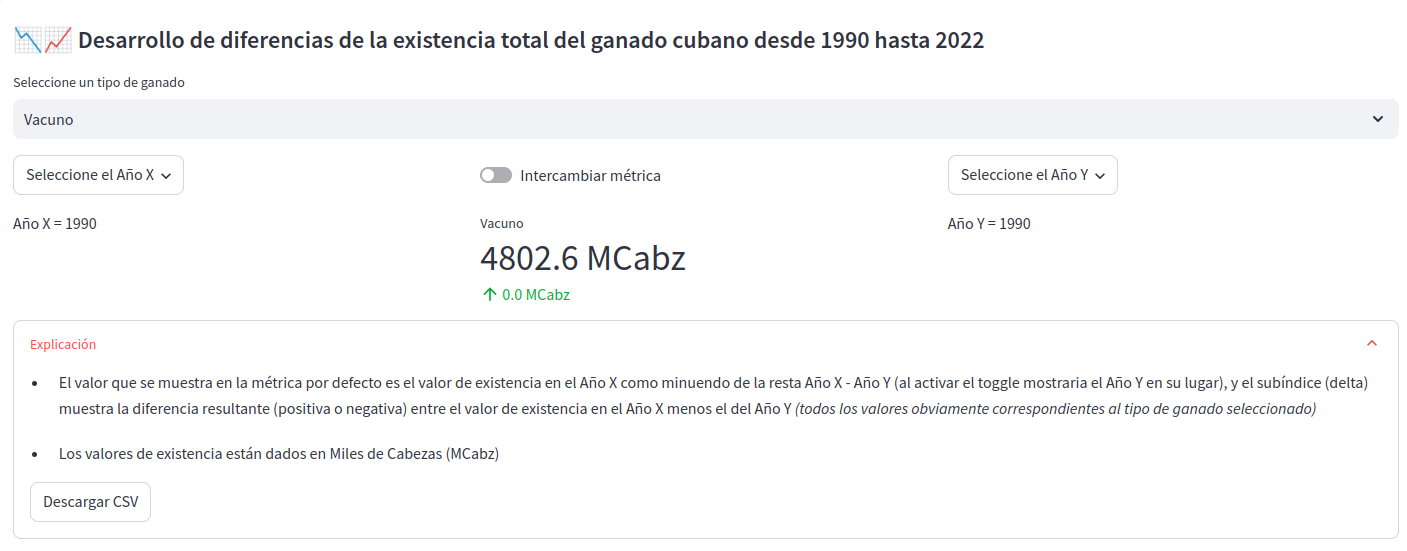
\includegraphics[width=1.0\textwidth]{img/metrics.png}
Por medio de esta representación se facilitaron los cálculos de las diferencias entre dos años para llegar a resultados como por ejemplo que con respecto a 1990 en 1995 se 
resulta en una diferencia de -170.6 MCabz de ganado vacuno producto de los efectos de la crisis de los 90, pero, por otro lado, en 1998 con respecto al 1995 se tiene un 
ligero incremento de +11.7 MCabz, que fue el período de recuperacióm post-crisis en la isla.
\subsubsection{Existencias del ganado por tipos y sectores}
Resulta necesario considerar evaluar por comparaciones para identificar patrones, tendencias y tomar decisiones de forma acertada de forma general en cualquier aspeceto. Por
esta razón se plantearon representación interactivas para dividir el análisis por sectores (generalmente en total, estatal  y no estatal) y por grupos de sexo, especies o 
tipos de ganado cuando se necesito excluir algun grupo.\\

De esta forma se encontraron patrones en las existencias por tipos de rebaño:
\begin{center}
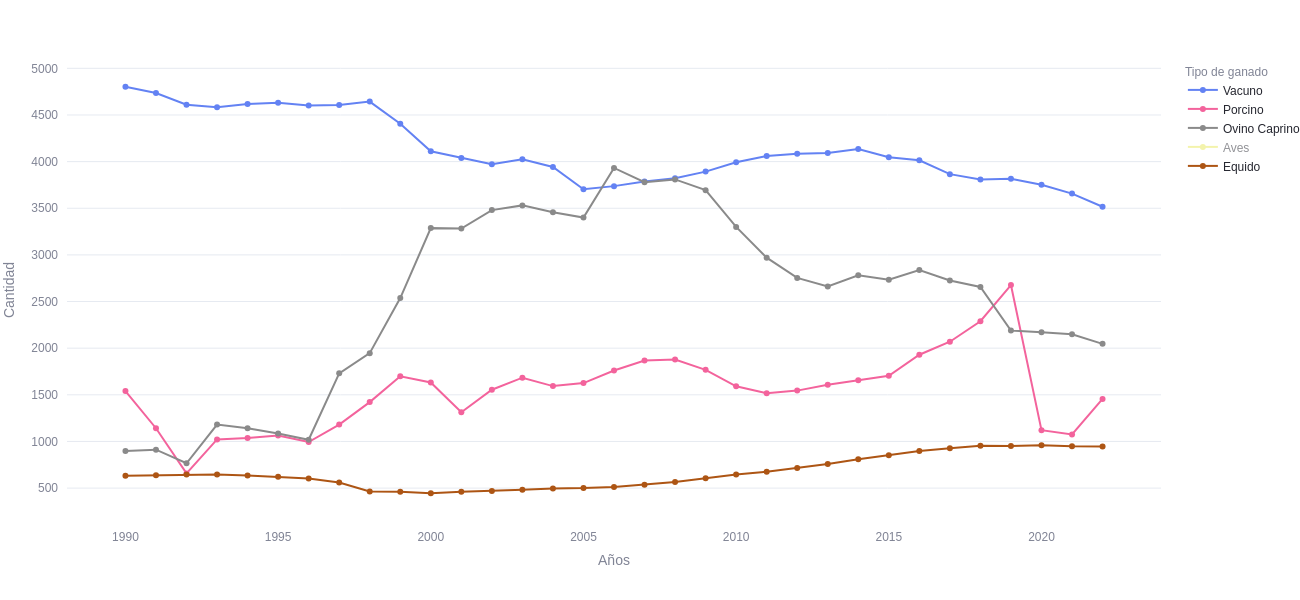
\includegraphics[width=1.0\textwidth]{img/2.png}
\end{center}
Se considera excluir a las aves por el crecimiento de escala que produce al ser mayores en cantidades de ganado menor. Y se observa una superioridad general del rebaño de bovino
con respecto al resto, exceptuando 2005-2010 que fueron los resultados producto de que el gobierno cubano comenzó a fomentar más la producción de leches de cabra y carne de cordero 
y cabra debido a su menor dependencia de importaciones.\\

Luego, aislandolos por tipos de ganado productores principales:
\begin{center}
    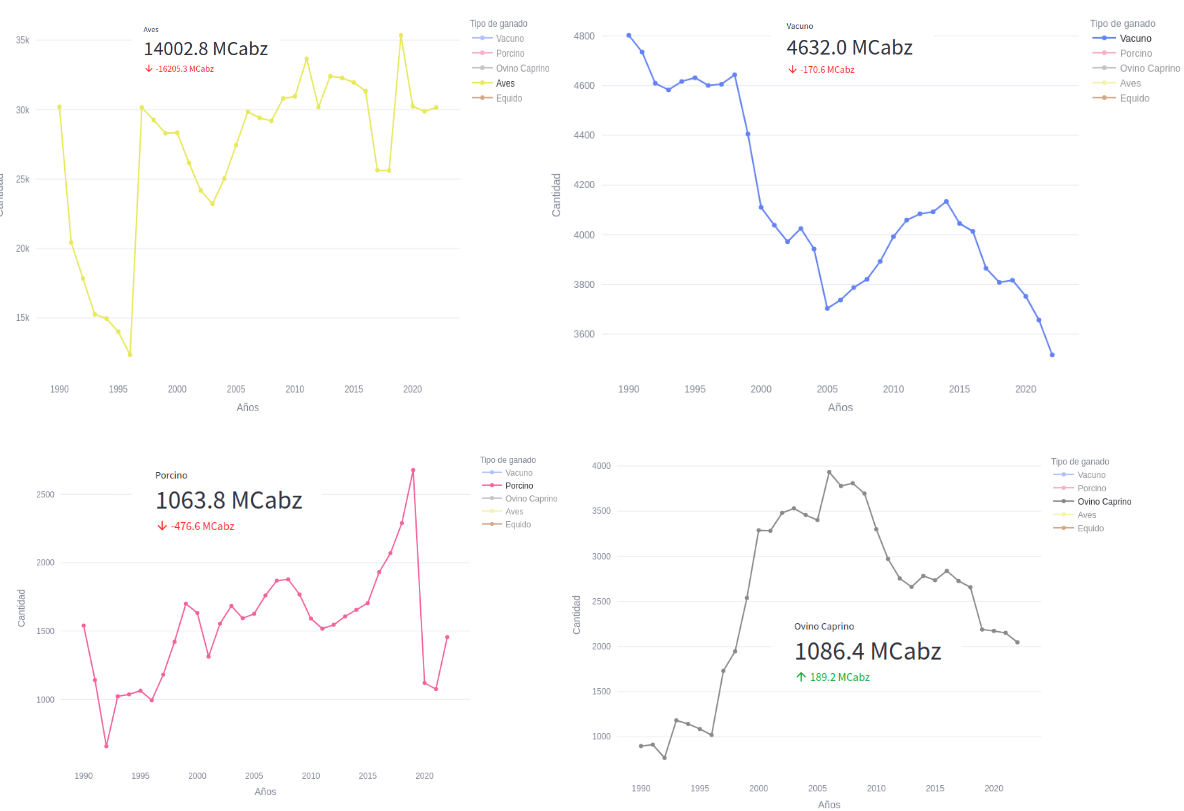
\includegraphics[width=1.0\textwidth]{img/plots_exist.png}
\end{center}
Se logran apreciar (con distribución de colores de amarillo para aves, azul para bovinos, rosa para porcinos y gris para ovino-caprinos por si no se alcanza a ver) varias cosas:
\begin{itemize}
    \item Una caída desproporcional para el sector de las avícola y bovino durante el período de 1990-1995 como parte de la crisis (los vacunos se mantuvieron mucho mas estables en comparación y hubo hasta un ligero crecimiento para el 1994).
    \item Un crecimiento casi vertical del grupo de las aves como resultado del período de recuperación que casi triplico la existencia de aves. El resto de rebaños tambien tuvieron un incremento en este período.
    \item Unas lineas de crecimiento estables para los porcinos y ovino-caprinos. Estos sectores presentaron un comportamiento diametralmente opuesto al resto. Mientras que el ganado bovino y avícola continuaba sufriendo una reducción en las 
    entregas de sacrificio y existencias de forma períodica, estos lograron mantenerse estables, incluso, experimentar un crecimiento sostenido hasta el año 2018 para los porcinos y 2006 para los ovinos-caprinos. Esta disparidad entre los diferentes 
    tipos de ganado refleja las particularidades de cada sector dentro del contexto económico cubano. Históricamente han sido los resistente a las condiciones adversas. 
    \item El decrecimiento general constante del ganado vacuno, sólo en recuperación en los años 2005 hasta 2014.
    \item Las pérdidas generales para finales de la segunda decada y comienzos de la tercera del 2000 (exceptuando a los equidos excluidos que mantuvieron su crecimiento). Producto de los simultaneos cambios económicos y condiciones climáticas y epidemiologicas por los que fue atravesando el país 
\end{itemize}

De igual forma para las entregas a sacrificio se mantuvieron patrones generalmente similares a los de existencia, exceptuando por los ovino-caprinos que de las fuentes de la ONEI se desconocen los valores hasta 2007.
Probablemente producto de aquellos años de intensificación de la producción y reproducción de este tipo de rebaño.\\
\newpage
\subsubsection{Producción}
Dentro de este apartado, comenzando con la producción de leche, se logran percibir las siguientes particularidades principales:
\begin{center}
    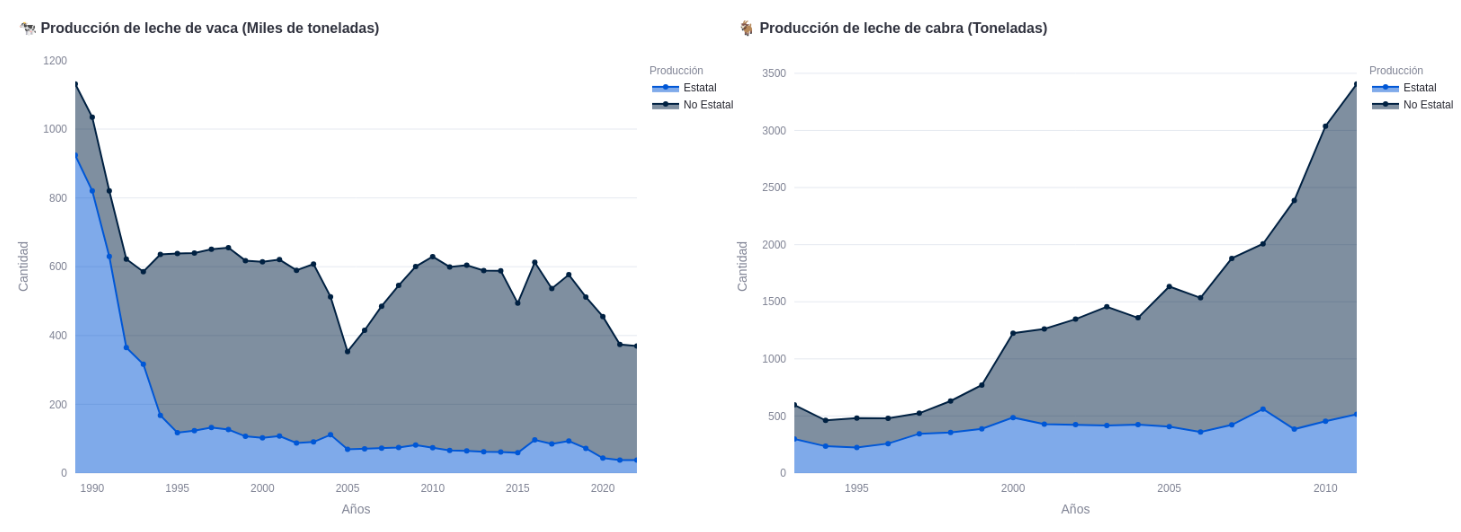
\includegraphics[width=1.0\textwidth]{img/lechee.png}
\end{center}
\begin{itemize}
    \item Predominio del sector no estatal para ambos grupos a partir del 93 para los vacunos y 99 para las cabras, como resultante de la flexibilización de las regulaciones sobre la producción y comercialización de productos lácteos por parte del gobierno cubano, 
    permitiendo a los productores no estatales operar más libremente.
    \item Disminución general vacuna y crecimiento casi constante en cabras. 
\end{itemize}
Sin embargo, el rendimiento anual de vacas de ordeño se mantuvo relativamente semejante en ambos sectores desde 1993, anteriormente se tenían menos libertades para con el rebaño por lo que impería el sector estatal.\\\\
Por otro lado, con respecto a los huevos, su producir tuvo un recorrido general estable y tendiendo al crecimiento hasta la segunda mitad de la segunda década de los años 2000 (exceptuando el período de decrecimiento monstruoso de los 90 por la crisis). Desde ese momento en adelante se ha mantenido oscilando la línea de su desarrollo, principalmente producto de la intensificación del hurto, los sacrificios, la caza y demás factores.
\begin{center}
    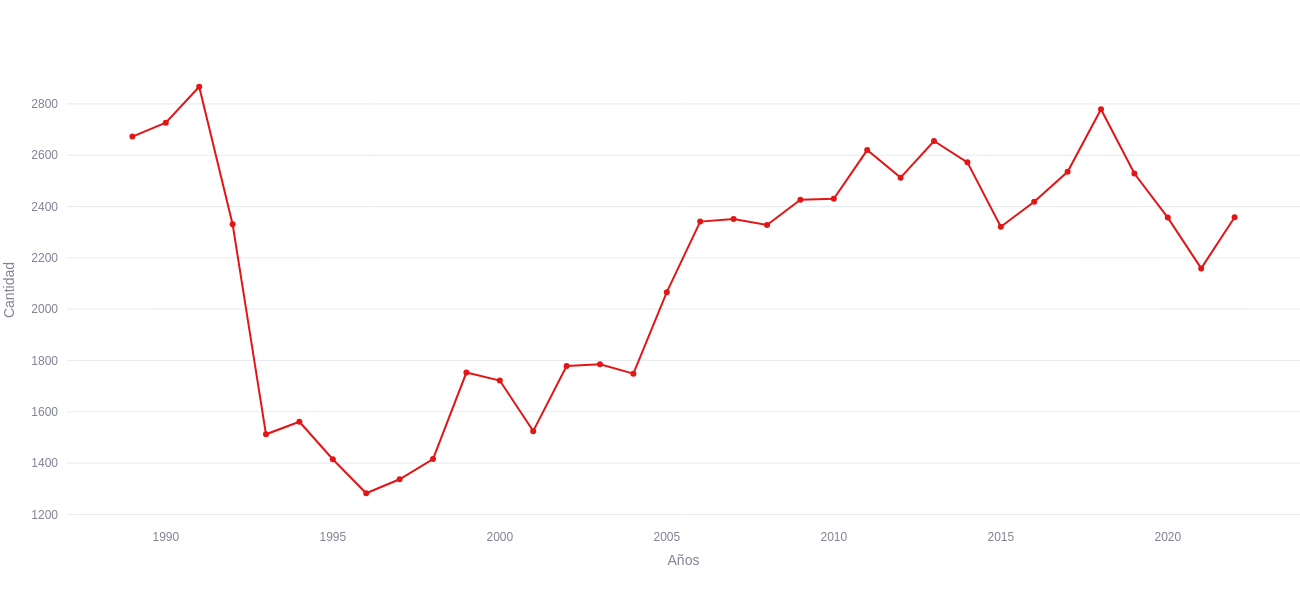
\includegraphics[width=1.0\textwidth]{img/11.png}
\end{center}
La producción de carne en general sufrió fue uno de las consecuencias de los valores de existencia y entregas a sacrificio de forma general, siguiendo una línea de disminución por todos los factores influyentes en la isla.
\newpage
\subsubsection{Alimentación}
Acerca de este tema, las fuentes principales de forma general se centraban en los residuos de caña, miel, urea, cachaza, el agua, y la mayor problemática hoy en día, el pienso.
\begin{center}
    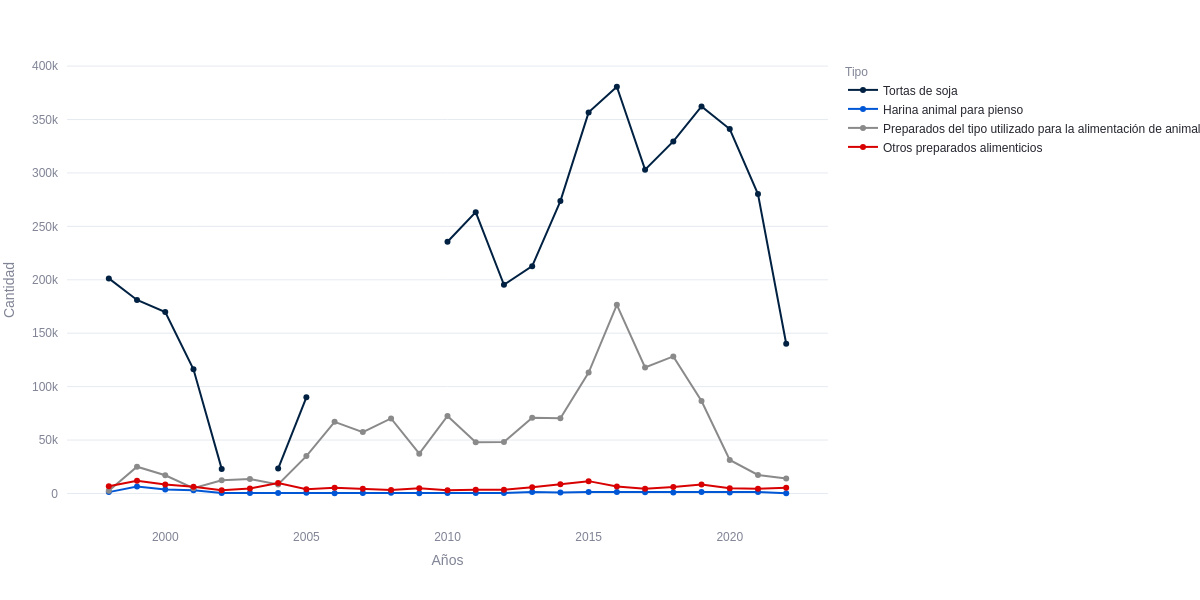
\includegraphics[width=1.0\textwidth]{img/1.png}
\end{center}
Para años posteriores a la crisis, con las diferentes relaciones, acuerdos y demás medidas del país se han logrado conseguir algunas fuentes de entrada pero de la misma manera ha subido el valor, por el exceso de demanda de después de la crisis, por lo que la situación 
para los productores no ha sido particularmente sencilla. Y además para despues del 2016 la situación vuelve a decaer producto de intentos del país de diversificar su economía y de complejidades burocráticas con su valor.
\subsubsection{Entidades}
Una de las medidas principales en el campo agrícola fue el surgimiento de la Cooperativa de Crédito y Servicio (CCS) como una herramienta estatal para organizar la producción de los pequeños propietarios rurales y integrarlos activamente en la vida política 
del país. La Asociación Nacional de Agricultores Pequeños (ANAP) jugó un papel crucial en la promoción y apoyo a estas cooperativas. Posteriormente, en el periodo 1975-1985 se expandió la industrialización de la economía cubana, estimulada por la cooperación 
con los países del campo socialista. Como parte de ese proceso, en el Primer Congreso del Partido Comunista de Cuba (PCC) (1975) se planteó como prioridad acelerar el movimiento cooperativo, pero sobre todo encaminarlo a la integración de los campesinos de las 
CCS a lo que se denominó CPA, las cuales socializan los medios de producción, entre ellos la tierra, que deja de ser propiedad privada individual y pasa a ser propiedad colectiva. Tiempo después como contramedida a las repercusiones de la próxima crisis económica de 
1990 se fundan las Unidades Básicas de Producción Cooperativa (UBPC), constituidas en 1993

\clearpage
Desde ese instante se mantuvo dicha estructura hasta el 2011 que surgen las Cooperativas no Agropecuarias para asentarse en el 2013.
\begin{center}
    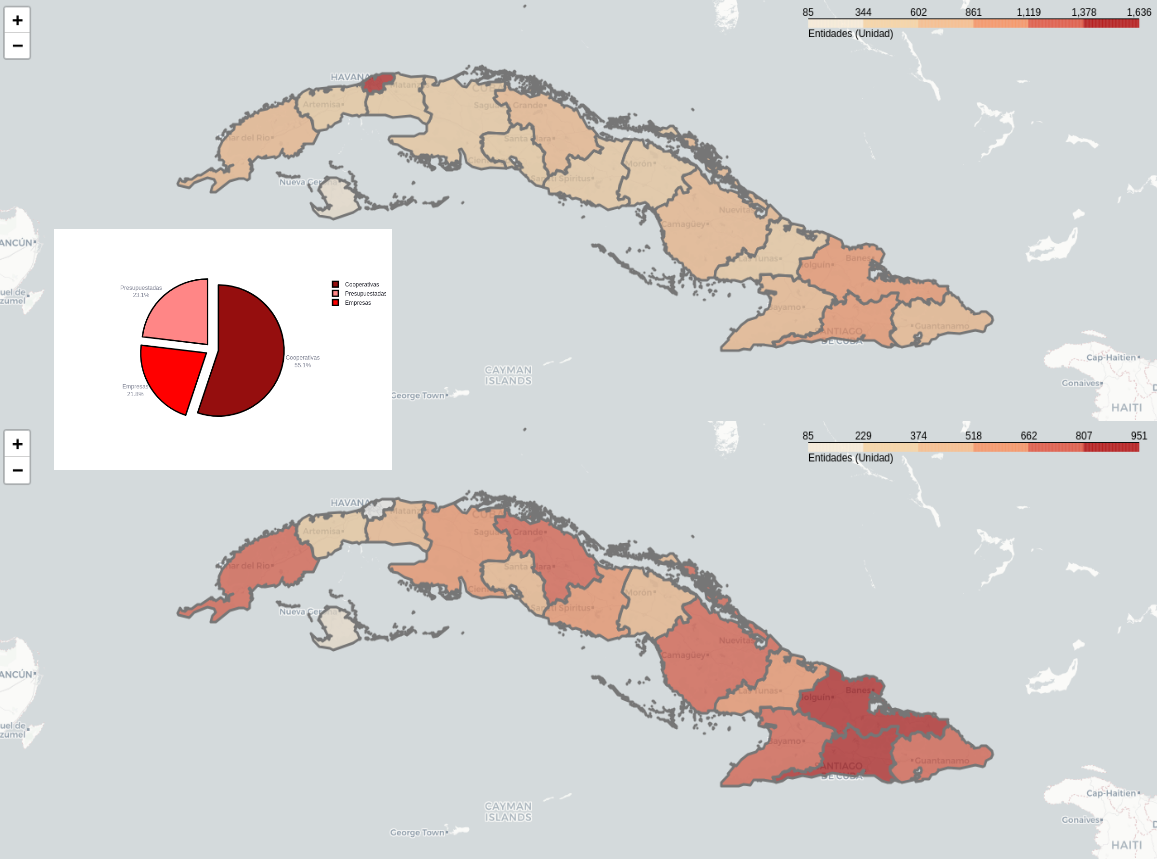
\includegraphics[width=1.0\textwidth]{img/mapa.png}
\end{center}
Cómo se puede observar en el mapa, la distribución espacial de las instituciones de forma general siempre ha estado concentrada en la capital, y, al excluirla, se aprecia como estas entidades se concentran en mayores cantidades hacia la zona más oriental del país (y Camagüey),
Pinar del Río y Villa Clara en la zona central. Y con una concentración general de un 46,5\%, 35,6\% y 17.1\% de CCS, UBPC y CPA respectivamente para un total de 5688 unidades cooperativas en el año 2012.

\section{Conclusiones y recomendaciones}
Concluyendo el análisis sobre la ganadería en Cuba, podemos afirmar que el sector enfrenta desafíos significativos pero también oportunidades para su desarrollo. Por un lado, Cuba ha logrado ciertos avances en la producción de carne y productos lácteos, lo que sugiere una cierta 
resiliencia del sistema agropecuario. Sin embargo, la dependencia de importaciones y el déficit alimentario persisten como problemas estructurales que requieren atención urgente.

Para mejorar la situación de la ganadería cubana, se recomiendan estrategias de diversificación productiva, inversión en tecnologías y prácticas sostenibles, y fomento del desarrollo rural. Además, es crucial fortalecer las capacidades técnicas y empresariales de los productores, 
así como mejorar la infraestructura agrícola y ganadera. También sería beneficioso revisar y ajustar políticas públicas para alinearlas más estrechamente con las necesidades y posibilidades del sector privado, potenciando su contribución al desarrollo económico y social del país. 
Finalmente, se debe abordar la transición hacia una economía más circular y resiliente, aprovechando recursos locales y reduciendo la dependencia de importaciones, lo cual podría llevar a una mayor autosuficiencia alimentaria y a una industria ganadera más robusta y competitiva.
\end{document}
